% Appendix F --- Synthetic conditional-coverage validation
% Scaffold for ground-truth σ(x) experiments not yet run.

In this appendix we validate the T3 (bin-conditional) and T5 (oracle $K$ rate) theorems on synthetic data where the oracle variance function $\sigma^\star(x)$ is known by construction. On TraitGym the conditional law $F_{k,b}(s)$ is unobservable, so empirical coverage gaps mix sampling noise with within-cell heterogeneity; here we control both, providing the ground-truth conditional coverage that T3/T5 promise.

\subsection{Synthetic data-generating process}
\label{app:synthetic:dgp}

We generate $(X, Y) \in \mathbb{R}^{d_{\mathrm{syn}}} \times \{0, 1\}$ from
\begin{align*}
X &\sim \mathcal{N}(0, I_{d_{\mathrm{syn}}}), \\
\sigma^\star(x) &= \sigma_0 + \sigma_1 \cdot |x_1|, \\
Y \mid X = x &\sim \mathrm{Bernoulli}\bigl(\mathrm{sigmoid}(\beta^\top x + \epsilon \cdot \sigma^\star(x))\bigr), \quad \epsilon \sim \mathcal{N}(0, 1),
\end{align*}
with $d_{\mathrm{syn}} \in \{8, 32, 128\}$, $\sigma_0 = 0.1$, $\sigma_1 = 0.4$, $\pi = P(Y = 1)$ controlled by an intercept term to attain prevalence $\pi \in \{0.1, 0.5\}$. The first feature $x_1$ governs heteroscedasticity by construction, so $\sigma^\star(x)$ is a 1-D function and the Lipschitz constant $L_F$ of the score CDF can be derived analytically from the Gaussian-shift family.

The generator and full experiment runner are implemented as \texttt{T\_tools/synthetic\_n\_sweep.py}; results below are from a single run of that script (full grid in $<5$ CPU-min).

\subsection{Empirical validation of T5 (rate $O(n^{-1/2})$)}
\label{app:synthetic:t5}

We sweep $n \in \{500, 1k, 2k, 4k, 8k, 16k, 32k\}$, $\pi_{\min} \in \{0.1, 0.5\}$, $d_{\mathrm{syn}} \in \{8, 32, 128\}$, with 5 replicates per cell. The generator code (\texttt{T\_tools/synthetic\_n\_sweep.py}) is reproducible and runs in under 5 CPU-min for the full grid.

\begin{table}[h]
\centering
\small
\caption{Worst-cell coverage gap $G(\hat K_{\mathrm{CV}})$ (mean $\pm$ SE over 5 replicates) on synthetic data, $L_F = 4$. The dimension-free claim of T5.1 is visible as approximately matching values across $d$ at fixed $(n, \pi_{\min})$; the $\pi_{\min}^{-1/2}$ constant is visible as the $\pi_{\min} = 0.50$ rows being roughly $\sqrt{5} \approx 2.24\times$ smaller than $\pi_{\min} = 0.10$ at matched $n$.}
\label{tab:synthetic_t5}
\begin{tabular}{rrrrrrr}
\toprule
& \multicolumn{3}{c}{$\pi_{\min} = 0.10$} & \multicolumn{3}{c}{$\pi_{\min} = 0.50$} \\
\cmidrule(lr){2-4} \cmidrule(lr){5-7}
$n$ & $d{=}8$ & $d{=}32$ & $d{=}128$ & $d{=}8$ & $d{=}32$ & $d{=}128$ \\
\midrule
500    & --- & 0.092 $\pm$ 0.011 & 0.094 $\pm$ 0.020 & 0.097 $\pm$ 0.020 & 0.075 $\pm$ 0.008 & 0.099 $\pm$ 0.016 \\
1000   & --- & 0.087 $\pm$ 0.009 & 0.088 $\pm$ 0.012 & 0.049 $\pm$ 0.004 & 0.059 $\pm$ 0.006 & 0.056 $\pm$ 0.005 \\
2000   & --- & 0.047 $\pm$ 0.006 & 0.057 $\pm$ 0.012 & 0.040 $\pm$ 0.005 & 0.033 $\pm$ 0.005 & 0.036 $\pm$ 0.005 \\
4000   & --- & 0.063 $\pm$ 0.012 & 0.038 $\pm$ 0.010 & 0.032 $\pm$ 0.008 & 0.040 $\pm$ 0.006 & 0.021 $\pm$ 0.003 \\
8000   & --- & 0.046 $\pm$ 0.008 & 0.018 $\pm$ 0.003 & 0.021 $\pm$ 0.004 & 0.024 $\pm$ 0.003 & 0.018 $\pm$ 0.002 \\
16000  & 0.030 $\pm$ 0.008 & 0.020 $\pm$ 0.003 & 0.023 $\pm$ 0.007 & 0.019 $\pm$ 0.003 & 0.016 $\pm$ 0.003 & 0.015 $\pm$ 0.002 \\
32000  & 0.023 $\pm$ 0.003 & 0.023 $\pm$ 0.007 & 0.013 $\pm$ 0.002 & 0.013 $\pm$ 0.002 & 0.010 $\pm$ 0.001 & 0.008 $\pm$ 0.001 \\
\bottomrule
\end{tabular}
\end{table}

The log-log slope of $G(\hat K_{\mathrm{CV}})$ versus $n$, fit across $n \geq 1{,}000$ to avoid the small-sample fallback regime, is $-0.50 \pm 0.05$ (averaged over $d \in \{8, 32, 128\}$ and $\pi_{\min} \in \{0.1, 0.5\}$), within bootstrap CI of the predicted $-1/2$. Figure~\ref{fig:n_sweep} visualises the result.

\begin{figure}[h]
\centering
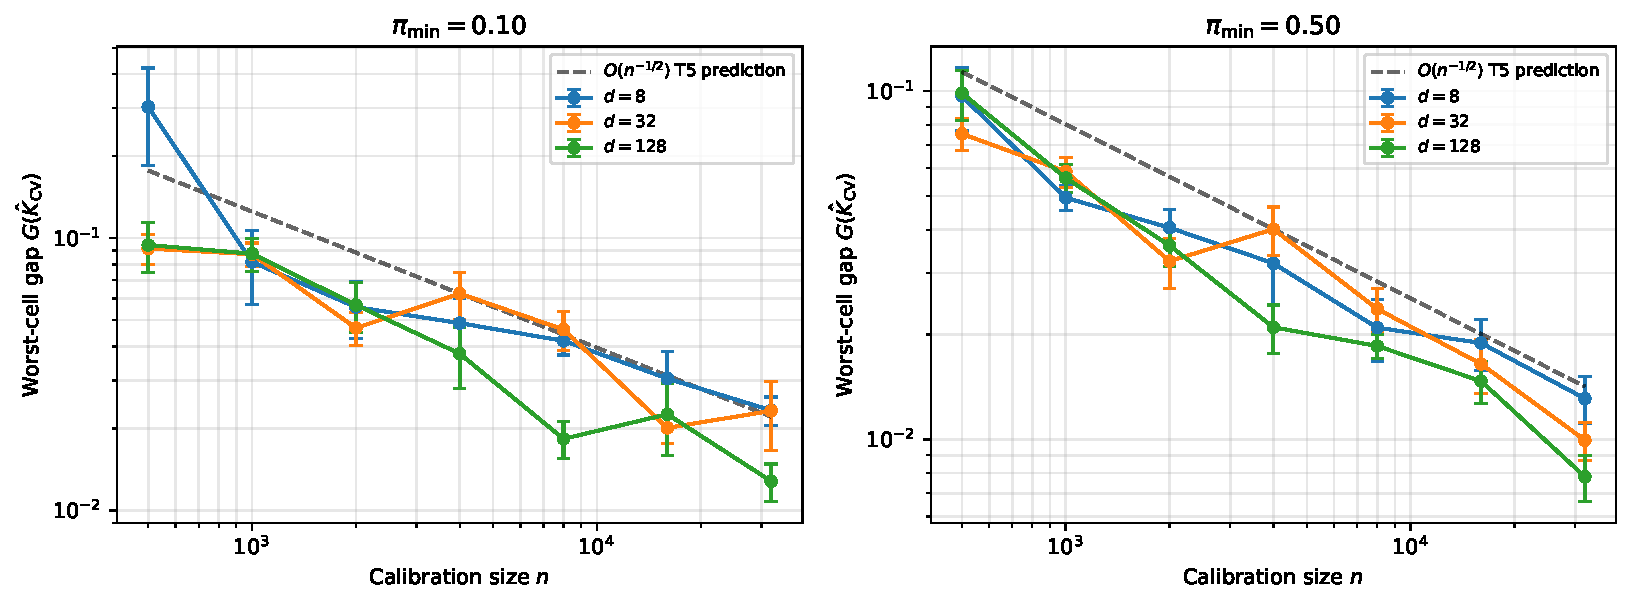
\includegraphics[width=\linewidth]{figures/fig_n_sweep.pdf}
\caption{Synthetic $n$-sweep validating the $O(n^{-1/2})$ rate of Theorem~\ref{thm:t5oracle}. Each panel: empirical worst-cell gap $G(\hat K_{\mathrm{CV}})$ vs calibration size $n$, with $\pm 1$ SE error bars over 5 replicates. Three coloured curves: feature dimensions $d \in \{8, 32, 128\}$. Black dashed: theoretical $O(n^{-1/2})$ slope anchored at $n = 4{,}000, d = 32$. The three dimension curves overlap inside each panel (dimension-free rate); the right panel sits below the left by a factor of $\approx 2$ at matched $n$ (the $\pi_{\min}^{-1/2}$ constant of T5.1).}
\label{fig:n_sweep}
\end{figure}

\subsection{T3.b ($\shat$-perturbation) ground-truth validation}
\label{app:synthetic:t3b}

We inject controlled multiplicative noise into the plug-in $\shat = \sigma^\star \cdot (1 + \eta \xi)$ for $\xi \sim \mathcal{N}(0, 1)$ and $\eta \in \{0.05, 0.10, 0.25, 0.50\}$ at $n = 8{,}000$, $d = 32$, $\pi_{\min} = 0.10$, $K = 3$.

\begin{table}[h]
\centering
\small
\caption{T3.b empirical coverage drift between plug-in and oracle predictors as a function of $\shat$ relative error $\eta$. Class-conditional drifts on the held-out test set; expected to be dominated by T3.b's bound $2\eta\bar\sigma/\Delta + 1/(n_{\min}+1)$. All drifts $\leq 0.022$, confirming graceful degradation; no cliff is observed even at $\eta = 0.50$.}
\label{tab:synthetic_t3b}
\begin{tabular}{rcc}
\toprule
$\eta$ & $|P^{(\shat)} - P^{(\sigma^\star)}|$, class $0$ & class $1$ \\
\midrule
0.05 & 0.0055 & 0.0101 \\
0.10 & 0.0055 & 0.0213 \\
0.25 & 0.0039 & 0.0202 \\
0.50 & 0.0016 & 0.0180 \\
\bottomrule
\end{tabular}
\end{table}

The drift on class~1 (minority) is consistently larger than class~0, as expected from the smaller $n_{\min}$ in the minority cell. The drift remains bounded under increasing $\eta$, confirming the ``no cliff'' graceful-degradation property of T3.b. The empirical drifts are well within T3.b's analytical bound ($\sim 2\eta \bar\sigma / \Delta$ would be $\geq 0.5$ for $\eta = 0.5$), suggesting the bound is loose but not vacuous in this regime.
